\documentclass[10pt,onecolumn]{book}

\usepackage{times} % font
\usepackage{graphicx} % picture reference
\usepackage{amsmath} % split of mathematical formulas
\usepackage{amssymb} % special mathematical symbols
\usepackage{geometry} % margin
\usepackage{setspace} % letter-spacing
\usepackage{indentfirst} % indent
\geometry{left=2cm,right=2cm, top=2cm, bottom=2cm}
\usepackage{hyperref} % hyperlink
\usepackage{cite}
\usepackage[sectionbib]{chapterbib}

\usepackage{multirow}
\usepackage{color}
\usepackage{ulem}
\usepackage{todonotes}

%\usepackage{fancy}%页眉页脚包
%\pagestyle{plain}%页眉页脚设置
\usepackage{fancyhdr}
\pagestyle{fancy}


\def\ie{\emph{i.e.}}
\def\eg{\emph{e.g.}}
\def\etal{\em {et al.}}

\newcommand{\bm}[1]{\mbox{\boldmath{$#1$}}}
\newcommand{\figref}[1]{Fig. \ref{#1}}
\newcommand{\tabref}[1]{Tab. \ref{#1}}
\newcommand{\equref}[1]{(\ref{#1})}
\newcommand{\secref}[1]{Sect. \ref{#1}}
\newcommand{\algref}[1]{Alg. \ref{#1}}
\newcommand{\myPara}[1]{\vspace{.05in}\noindent\textbf{#1}}
\newcommand{\rev}[1]{\textcolor{blue}{#1}}
\newcommand{\rr}[1]{\textcolor{red}{#1}}
\newcommand{\cg}[1]{\textcolor{green}{#1}}
\newcommand{\bb}[1]{\textcolor{blue}{#1}}
\newcommand{\bl}[1]{\textbf{#1}}
\newcommand{\ul}[1]{\underline{#1}}
\newcommand{\mc}[1]{\mathcal{#1}}
\newcommand{\mb}[1]{\mathbb{#1}}

\begin{document}

\title{\textbf{Paper Reading}}
\author{Jinming Su}
\date{Last update: \today}

\maketitle

\thispagestyle{empty}
\newpage
\pagenumbering{Roman}
\newpage
\tableofcontents
%\newpage
%\listoffigures
%\newpage
%\listoftables
%\newpage
%\pagenumbering{arabic}
\newpage
\listoftodos

\newpage
\pagenumbering{arabic}
\mainmatter

\chapter{Classification}
\section{Res2Net: A New Multi-scale Backbone Architecture, arxiv, 2019.}
\begin{figure}[h]
\centering
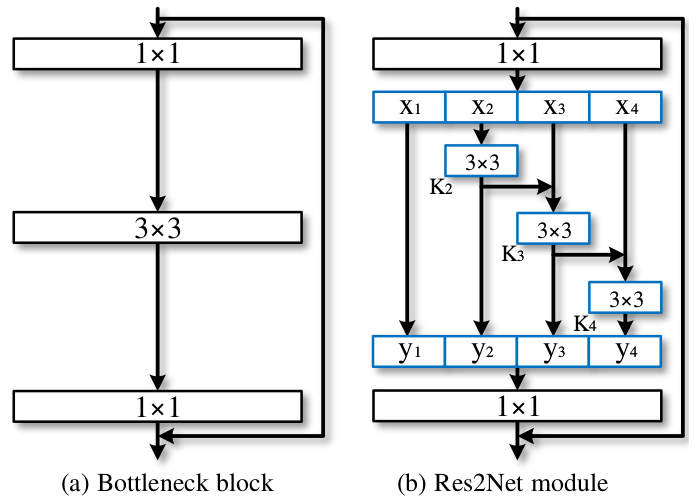
\includegraphics[width=0.4\textwidth]{figures_paper_reading/Res2Net:_A_New_Multi-scale_Backbone_Architecture.png}
\caption{Residual Learning.}
\label{fig:1-1_residual_learning}
\end{figure}
This paper is mainly a promotion of residual network, which seems to be similar to cardinality, only adding more connections.

\chapter{Object Detection}
\section{Proposal}
\subsection{Multiscale Combinatorial Grouping for Image Segmentation and Object Proposal Generation. TPAMI, 2016}
I don't read this paper, but the code is tested. Code can be found in \url{https://github.com/jponttuset/mcg}. When testing, run pre-trained/install.m, pre-trained/demos/demo\_im2mcg.m and get the following results.
\begin{figure}[h]
\centering
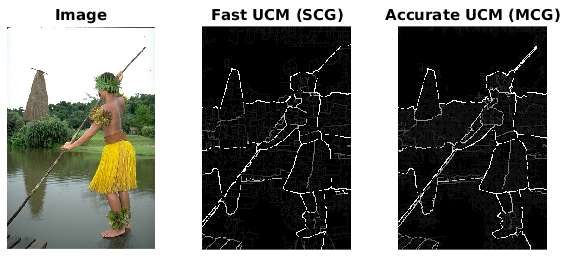
\includegraphics[width=0.6\textwidth]{figures_paper_reading/MCG_UCM.png}
\caption{The UCM of MCG.}
\label{fig}
\end{figure}

\begin{figure}[h]
\centering
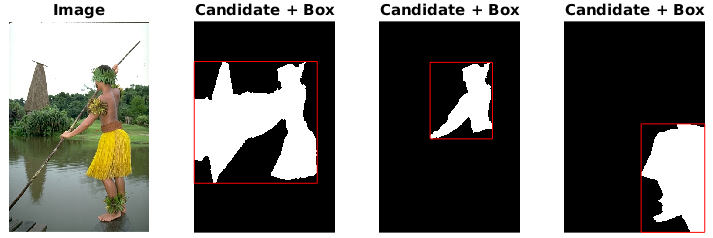
\includegraphics[width=0.8\textwidth]{figures_paper_reading/MCG.png}
\caption{The results of MCG.}
\label{fig}
\end{figure}

\section{What Object Should I Use? - Task Driven Object Detection. CVPR, 2019.}
\begin{figure}[h]
\centering
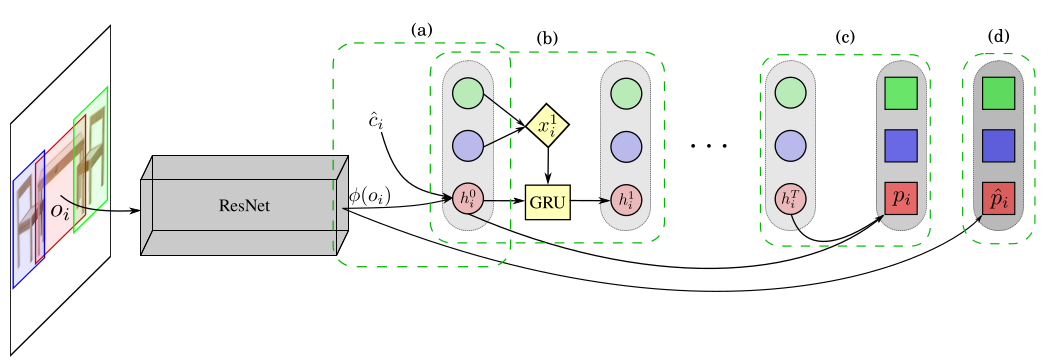
\includegraphics[width=0.8\textwidth]{figures_paper_reading/What_Object_Should_I_Use?_-_Task_Driven_Object_Detection.png}
\caption{GGNN.}
\label{fig}
\end{figure}

This paper has two contributions:
(1) construct a COCO-Tasks dataset which comprises about 40,000 images where the most suitable objects for 14 \uline{tasks} have been annotated;
(2) proposes a method buliding on \uline{Gated Graph Neural Network} to detect the most suitable objects for a given task. 

\section{Feature Pyramid Networks for Object Detection. CVPR, 2017.}
This paper propose a new backbone network.
\begin{figure}[h]
\centering
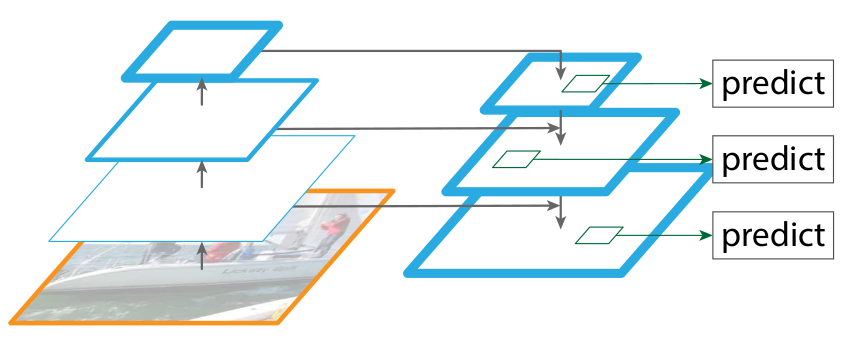
\includegraphics[width=0.4\textwidth]{figures_paper_reading/fpn.png}
\caption{Structure of FPN.}
\end{figure}

\section{Focal Loss for Dense Object Detection. ICCV, 2017}
This paper propose a improved cross entropy loss.

\begin{equation}
\mathcal{FL}(p, y) =
\left\{
\begin{split}
- \alpha (1-p)^\gamma \log(p), \quad y = 1 \\
- (1-\alpha) p^\gamma \log(1-p), \quad y = 0
\end{split}
\right.
\end{equation}
where $\alpha$ is the weighting factor for class imbalance, and $p_t$ is the confidence 

\chapter{Salient Object Detection}
\section{DNA: Deeply-supervised Nonlinear Aggregation for Salient Object Detection. arxiv, 2019.}
\begin{figure}[h]
\centering
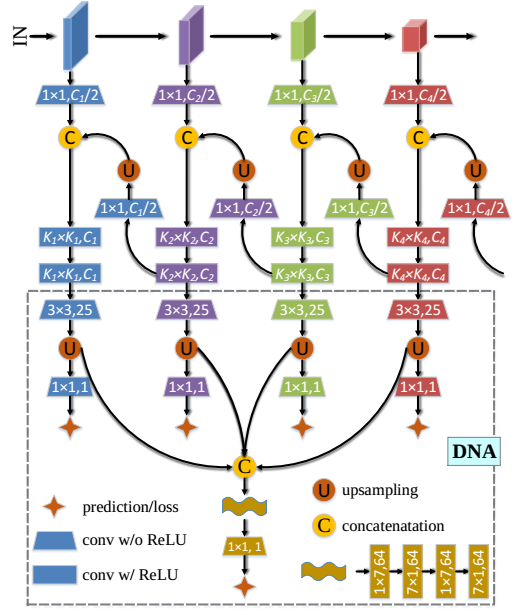
\includegraphics[width=0.4\textwidth]{figures_paper_reading/DNA_Deeply-supervised_Nonlinear_Aggregation_for_Salient_Object_Detection.png}
\caption{Residual Learning.}
\end{figure}

This paper has two contributions: 
(1) \uline{theoretically and experimentally} analyzes the natural limitaion of traditional side-output aggregration which can only make limited use of multi-scale side-ouput informantion; 
(2) proposes Deeply-supervised nonlinear aggregration (DNA) for side-output features. 
(3) as experience, in DNA, convolution layers with kernels of $n \times 1$ and $1 \times n$ are used, which is proved to be effective. Moreover, authers claim that large kernel size in DNA can improve performance.

\section{Instance-Level Salient Object Segmentation. CVPR, 2017.}
\begin{figure}[h]
\centering
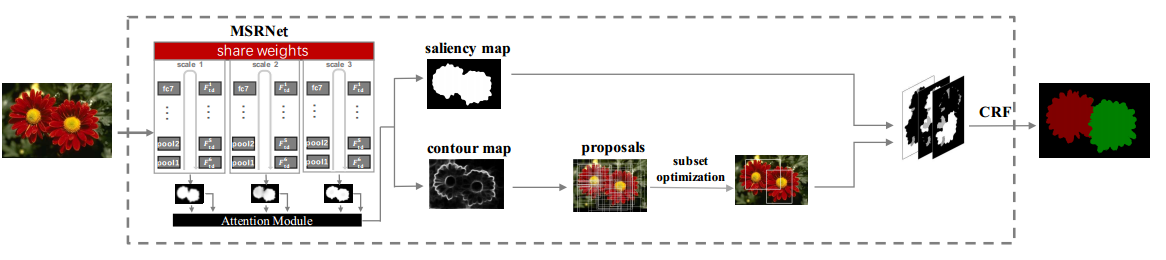
\includegraphics[width=1\textwidth]{figures_paper_reading/instance-SOD.png}
\caption{Instance-level salient object detection.}
\end{figure}

This paper has contributions as follows:
(1) introduce a new task of instance-level salient object detection, and construct a corresponding dataset with 1000 images that are collected from existing SOD datasets;
(2) propose a method for this task as shown in figure.

Moreover, the code can be found in \url{http://www.sysu-hcp.net/instance-level-salient-object-segmentation/}, while the code is only the part of SOD without contour and instance.

\section{Semantic Instance Meets Salient Object: Study on Video Semantic Salient Instance Segmentation. WACV, 2019.}

\section{A Simple Pooling-Based Design for Real-Time Salient Object Detection. CVPR, 2019}

\section{S4Net: Single Stage Salient-Instance Segmentation. CVPR, 2019.}

\section{Contrast Prior and Fluid Pyramid Integration for RGBD Salient Object Detection. CVPR, 2019}

\chapter{Semantic Segmentation}
\section{WebSeg: Learning Semantic Segmentation from Web Searches. arxiv, 2018.}
This paper propose a method to learning semantic segmentaion web searching images.
\begin{figure}[h]
\centering
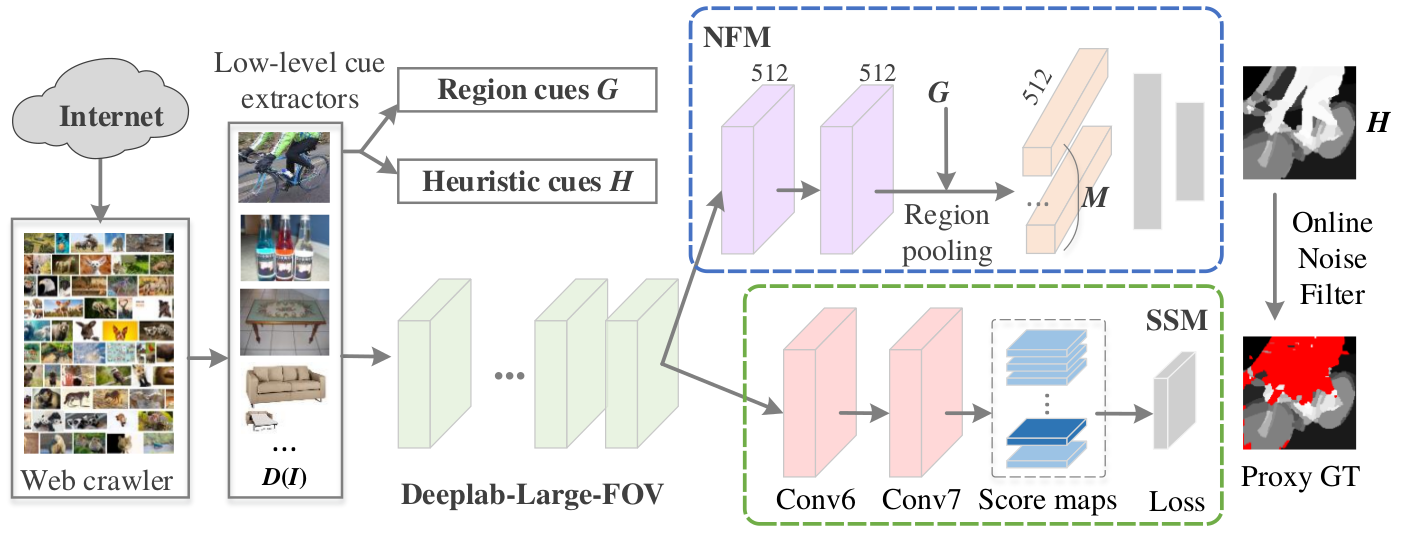
\includegraphics[width=0.8\textwidth]{figures_paper_reading/webseg.png}
\caption{Framework.}
\label{fig}
\end{figure}
The method is mainly an online noise filtering module, which is able to filter potentially noisy region labels to obtain the correct region labeled by the qury keywords.

\section{ADVENT: Adversarial Entropy Minimization for Domain Adaptation in Semantic Segmentation. CVPR, 2019.}
\begin{figure}[h]
\centering
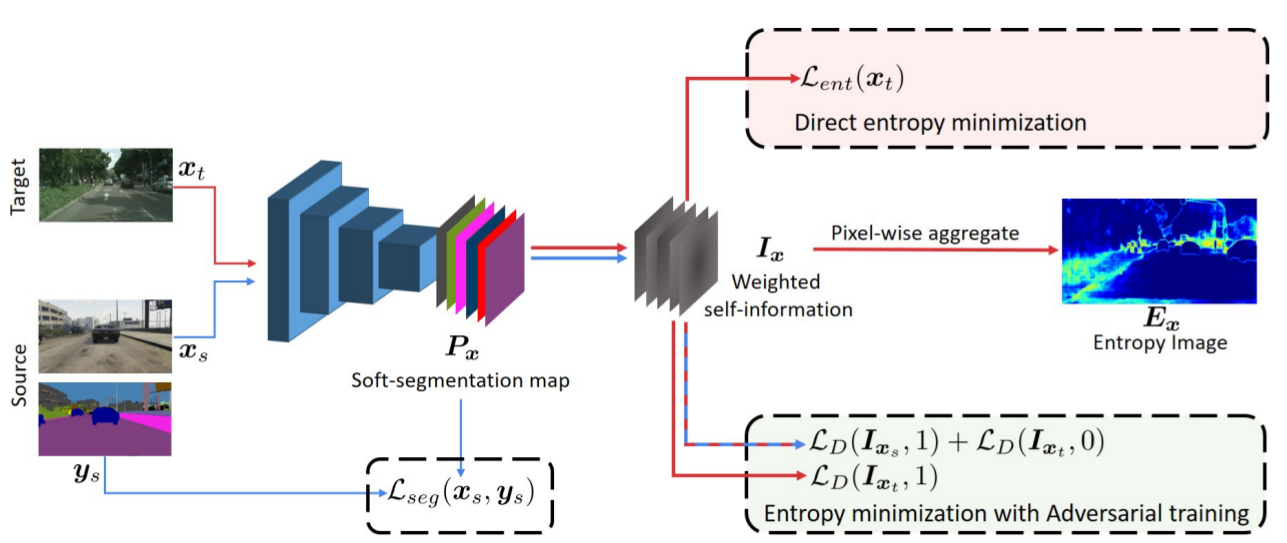
\includegraphics[width=0.8\textwidth]{figures_paper_reading/ADVENT_Adversarial_Entropy_Minimization_for_Domain_Adaptation_in_Semantic_Segmentation_CVPR2019.png}
\caption{Advsarial entropy.}
\label{fig}
\end{figure}
This paper focuses on the problem of domain adapation in semantic segmentation. In detail, the contributions are as follows: (1) propose to minimize the pixel-level entropy of target domain to penalize low-confident predictions on target domain; (2) propose a entropy-based adversarial traing approach to privide the structure adaptation; (3) extra two trick: a) training on specific entropy ranges and b) add class-ratio priors.

\section{Efficient Ladder-style DenseNets for Semantic Segmentation of Large Images. arxiv, 2019.}
\begin{figure}[h]
\centering
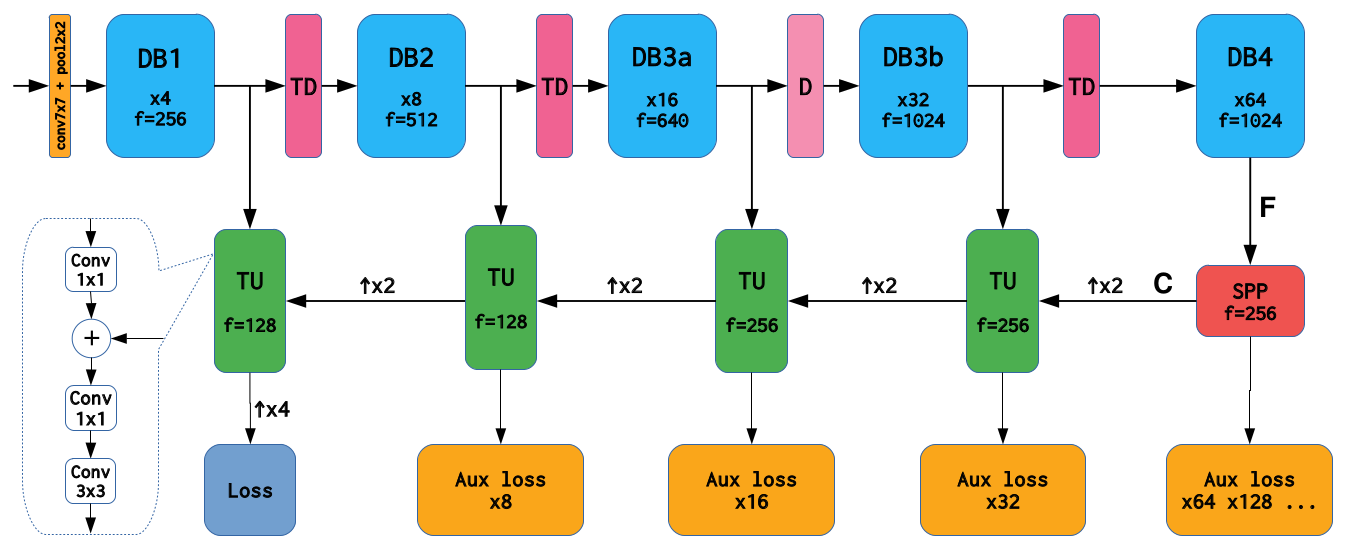
\includegraphics[width=0.8\textwidth]{figures_paper_reading/ladder_style_densenet.png}
\caption{Ladder-style densenet for semantic segmentation.}
\label{fig}
\end{figure}
This paper propose a ladder-style densenet for semantic segmentation, \uline{while I think this is not new idea, which has been widely used in present work such as FPN.} Moreover, this paper present to reduce the training memory footprint by aggressive re-computation of imtermediate activations during convolutional backprop, which maybe is worth learning. 

\chapter{Pose Estimation}
\section{DeepPose: Human Pose Estimation via Deep Neural Networks. CVPR, 2014.}
\begin{figure}[h]
\centering
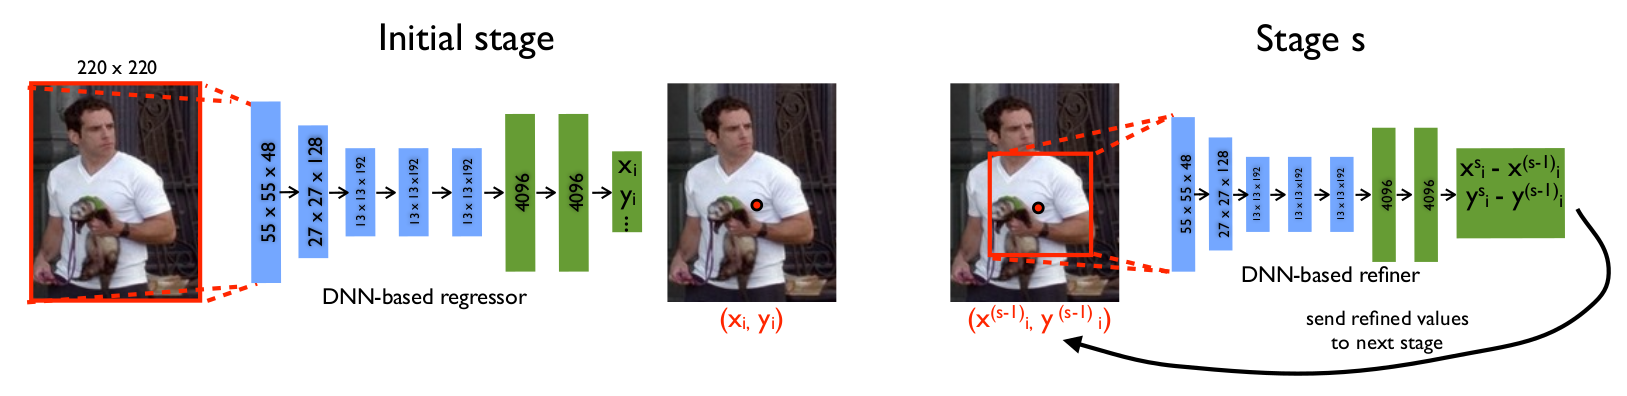
\includegraphics[width=1\textwidth]{figures_paper_reading/deeppose.png}
\caption{Deep pose.}
\label{fig}
\end{figure}
This method proposes a method to regress key points. It first predict these approximate locations, and then the box is croped, upsampled and sent to the regressor for the finer prediction.

\section{Human pose estimation via Convolutional Part Heatmap Regression. ECCV, 2016.}
\begin{figure}[h]
\centering
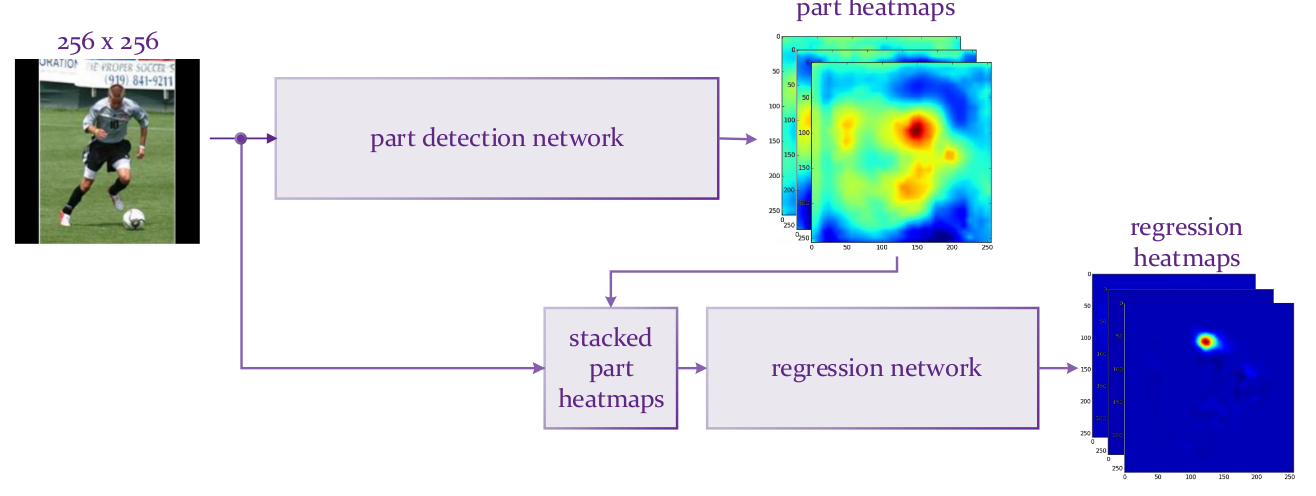
\includegraphics[width=0.8\textwidth]{figures_paper_reading/2016_ECCV_Human_pose_estimation_via_Convolutional_Part_Heatmap_Regression.png}
\caption{Convolutional part heatmap regression.}
\label{fig}
\end{figure}
This paper proposed the modern mainstream architecture by part heatmaps to solve the human pose estimation.

\section{Deep High-Resolution Representation Learning for Human Pose Estimation. CVPR, 2019.}
\begin{figure}[h]
\centering
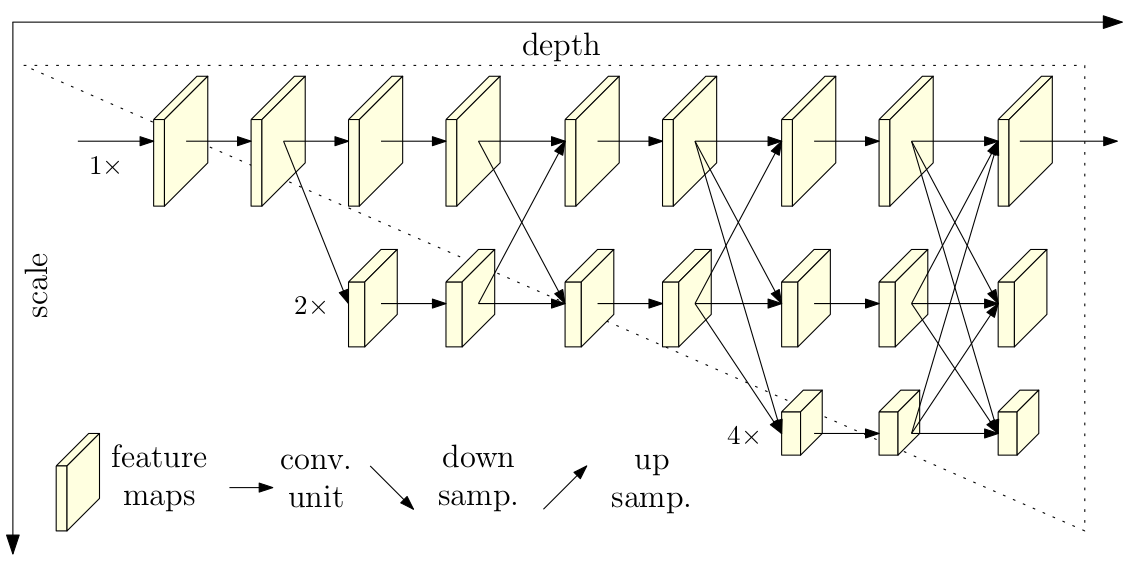
\includegraphics[width=0.8\textwidth]{figures_paper_reading/HRNet.png}
\caption{HRNet.}
\label{fig}
\end{figure}
This paper propose a new backbone network for maintaining high-resolution.

\chapter{Others}
\section{Single Image Haze Removal Using Dark Channel Prior. CVPR, 2009. Best paper.}
This paper introduces dark channel prior that is an observation -most local patches in haze-free outdoor images contain some pixels which have very low intensities in at least one color channel. \uline{This is the one of most famous papers in the domain of dehazing.}

Some formulas in this paper are easy to understand. One can refer to \url{https://www.cnblogs.com/Imageshop/p/3281703.html} for more understanding. 

The unofficial python code can be found in \url{https://github.com/su526664687/dark-channel-prior-dehazing}.

\section{Single Image Dehazing Using Ranking Convolutional Neural Network. TMM, 2018.}
\begin{figure}[h]
\centering
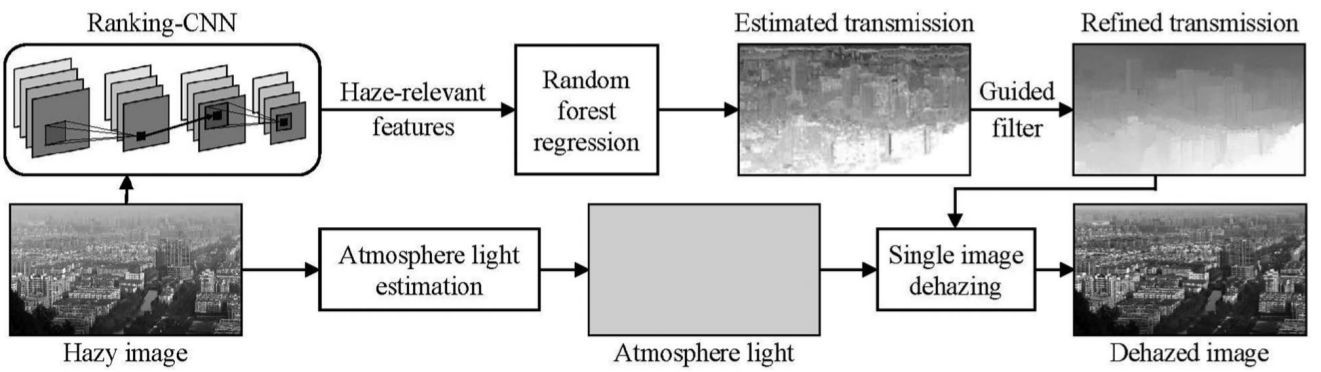
\includegraphics[width=0.8\textwidth]{figures_paper_reading/Single_Image_Dehazing_Using_Ranking_Convolutional_Neural_Network.png}
\caption{GGNN.}
\label{fig}
\end{figure}

This paper presents a ranking cnn to deal with dehazing. The ranking-cnn mainly means a ranking layer. In this layer, the values in a feature map are ranked, and the same operation is conducted for each feature map. Moreover, this paper introduce a method to synthesize haze images.

~\cite{su2019for}

{\small
\bibliographystyle{plain}
\bibliography{Ref_paper_reading}
}

\end{document}
